\chapter{A new strategy for the EMEP}
\label{Sec:Numerics}



\section{Introduction}
\label{Subsec:Numerics-intro}


This chapter presents \textit{the IRAM with adaptive parameter selection}, a new strategy for solving the EMEP by adaptively changing
the number of requested eigenvalues $r$ in the IRAM (Algorithm \ref{Alg:IRAM}).
Section \ref{Subsec:Numerics-adaptive_IRAM} develops the IRAM with adaptive parameter selection by examining the changing behavior of the IRAM across EMEP iterates.
Next, Section \ref{Subsec:Numerics-correl_btwn_EMEP_and_IRAM} closely examines the EMEP for two PLGD models with Gaussian noise (\ref{Eqn:PhaseLift-GD_Gaussian_noise}) to demonstrate an observed correlation between the clustering of the algebraically largest eigenvalues in the EMEP and an increase in the optimal choice of parameter $r$ in the IRAM.
We see that the IRAM with adaptive parameter selection properly tracks the optimal choice of $r$ for these models.
A more comprehensive set of performance results are presented in  Chapter \ref{Sec:Conclusion}.
Also note that all \emep \ experiments in this chapter are performed with Algorithm \ref{Alg:PGD} using the new termination conditions (\ref{Eqn:term_crit_new-primal_difference}) and (\ref{Eqn:term_crit_new-dual_difference}) established in Chapter \ref{Sec:PLGD_term_crit} and are available for reproduction.\footnote{\url{https://github.com/Will-Wright/low-rank-opt-rapid-eig}}








\section{The IRAM with adaptive parameter selection for the EMEP}
\label{Subsec:Numerics-adaptive_IRAM}



In this section we develop a new strategy for solving the \emep.  
This strategy uses the IRAM (Algorithm \ref{Alg:IRAM}) to handle each EMEP matrix iterate $A_k$ while adaptively changing one of the IRAM parameters based on the results from the EMEP iterates.
As discussed in Section \ref{Subsec:evol_mats-IRAM}, the IRAM has only two key parameters: the number of requested eigenvalues $r$ and the Arnoldi decomposition (\ref{Eqn:Arnoldi_decomp}) size $m$.
As we will see, the proper choice of these parameters can greatly reduce the number of matrix-vector products required for the EMEP.


We begin by examining the change in computational costs  (as measured by matrix-vector products) with respect to various \emep \ iterates $k$ and IRAM parameters $r$ in Figure \ref{Fig:Numerics-num_matvecs_orig_vs_optimal_params}.
In the original implementation of Algorithm \ref{Alg:PGD}, all EMEP iterates were handled using the IRAM with $r=2$ requested eigenvalues and Arnoldi decomposition size $m = \min \{  \max \{ 2r, 20 \}, n \}$, where $n$ is the size of the desired signal $x$.  
This choice of $m$ is equivalent to the default parameter setting in the IRAM solver \texttt{eigs} for MATLAB and evaluates to $m=20$ for $n \geq 20$.
Yet the plots in Figure \ref{Fig:Numerics-num_matvecs_orig_vs_optimal_params} demonstrate that choosing a fixed parameter $r=2$ can result in far more matrix-vector products than is optimal.


\begin{figure}[H]
\centering
\hbox{\hspace{-0.8cm} 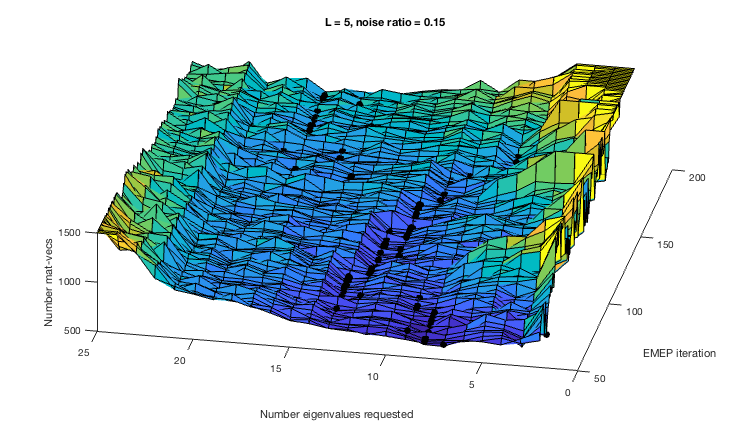
\includegraphics[scale=0.6]{Numerics-num_matvecs_orig_vs_optimal_params_1} }\vspace{1.0cm}
\hbox{\hspace{-1.6cm} 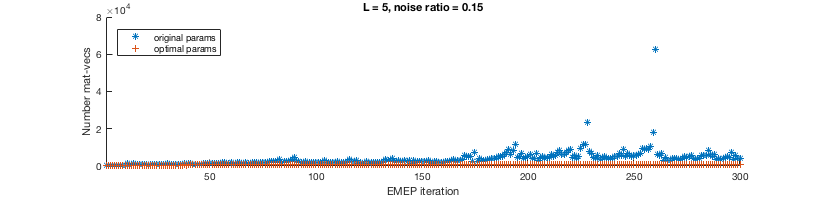
\includegraphics[scale=0.6]{Numerics-num_matvecs_orig_vs_optimal_params_2} }\vspace{0.0cm}
	\caption{
Performance results for an EMEP from a PLGD model with Gaussian noise	(\ref{Eqn:PhaseLift-GD_Gaussian_noise}) with noise ratio $\epsilon_\text{rel} = 0.15$, oversampling rate $L = 5$, and original signal from Figure \ref{Fig:parrot_signal_iterates} resized to $64 \times 64$ pixels.
Top: Number of matrix-vector products (capped at 1,500 for better viewing) for various EMEP iterates and number of requested eigenvalues $r$.  
Arnoldi decomposition size is set to $m = 40$ and black dots indicate the optimal parameter $r$ with the minimum number of products for each EMEP iterate.
Bottom: Plot of IRAM results for the EMEP with optimal parameters from top plot and fixed parameters $r=2$ and $m=20$.
	}
\label{Fig:Numerics-num_matvecs_orig_vs_optimal_params}
\end{figure}
% experiments.figure.noisyimage_adaptive_eig_full_exp




We now examine Figure \ref{Fig:Numerics-num_matvecs_orig_vs_optimal_params} to develop an adaptive strategy for choosing the number of requested eigenvalues $r$ for the sequence of EMEP iterates.
The top plot in Figure \ref{Fig:Numerics-num_matvecs_orig_vs_optimal_params} shows that the optimal choice of parameter $r$ typically changes only slightly between EMEP iterates.
However, the optimal parameter $r$ can increase quickly for later EMEP iterates (as we see around iterate 150 in the top plot in Figure \ref{Fig:Numerics-num_matvecs_orig_vs_optimal_params}).
Based on these observations, we may develop a strategy for choosing a sequence of parameters $r_1, r_2, \ldots, r_{maxit}$ as follows.
In order to measure change in the number of matrix-vector products for each iterate, we require that each pair of parameters $r_{k-1}$ and $r_k$ differ by at least one.
To select a new parameter $r_+$, we compare the two most recent choices for $r$ and the resulting number of matrix-vector products.
If these two choices for $r$ decreased the number of matrix-vector products, we continue to shift the value of $r$ in this direction by one unit; and otherwise we shift $r$ in the opposite direction.
We also allow $r$ to increase or decrease $r$ more rapidly by comparing the four most recent choices for $r$ and the resulting number of matrix-vector products using linear interpolation.
If these recent choices suggest the same shift as the first comparison, then we shift $r$ in this direction by two units rather than one.



This adaptive strategy for choosing the number of requested eigenvalues $r_k$ for each \emep \ iterate $k$ has the following steps.
First, we select a fixed Arnoldi decomposition size $m$ and initialize $r_1=r_{min}$ and $r_2 = r_1+1$ (where $r_{min}=2$, and $r_{max} = \min\{ 30, m-5 \}$, and we set the default value $m=40$).  
At each step $k \geq 2$ we update $r_{k+1} =  r_k + \delta$, where $\delta \in \{-2, -1, 1, 2\}$ is a shift based on the number of requested eigenvalues $r_k, r_{k-1}, \ldots$ and number of matrix-vector products $t_k, t_{k-1}, \ldots$ for the previous eigenvalues problems.
The shift $\delta$ is computed as follows.
First, we determine a \textit{$2$-step shift value} $\delta_2 \in \{-1, 1\}$ based on $r_{k-1}, r_k$ and $t_{k-1}, t_k$.
If $r_k > r_{k-1}$ and $t_k < t_{k-1}$ then the number of matrix-vector products in the \emep \ decreased as the number of requested eigenvalues was increased, suggesting we should shift $r_k$ by $\delta_2 = 1$.
By the same reasoning for the other three inequality cases, we define the
\textit{$2$-step shift value} as
\begin{equation}				\label{Eqn:adaptive_delta_2}
\delta_2 = \sign(r_k - r_{k-1}) \cdot \sign(t_{k-1} - t_k),
\end{equation}
where $\sign(0)$ is defined as $1$.
Next, if $k \geq 4$ then we compute a linear interpolation of the past four requested eigenvalue numbers and matrix-vector products by solving
\begin{equation} 			\label{Eqn:adaptive_delta_4_lin_interp_prob}
\min_{\alpha, \beta} || y - \alpha e - \beta x ||,
\end{equation}
where $y = [t_{k-3}; t_{k-2}; t_{k-1}; t_k]$ is the vector of matrix-vector product values, $x = [r_{k-3}; r_{k-2}; r_{k-1}; r_k]$ is the vector of the number of requested eigenvalues, and $e = [1;1;1;1]$.
If the solution to (\ref{Eqn:adaptive_delta_4_lin_interp_prob}) has $\beta > 0$ then the past four eigenvalue problems suggest that $t_i$ increases with $r_i$, and thus we should decrease $r_k$.
Thus we have the \textit{$4$-step shift value}
\begin{equation}			\label{Eqn:adaptive_delta_4}
\delta_4 = -\sign(\beta),
\end{equation}
where $\beta$ is determined by (\ref{Eqn:adaptive_delta_4_lin_interp_prob}).
If $\delta_2 = \delta_4$, then the $2$-step (\ref{Eqn:adaptive_delta_2}) and $4$-step equations (\ref{Eqn:adaptive_delta_4}) both suggest we should shift in the direction of $\delta_2$, and we select the shift $\delta = 2\delta_2$.
If $\delta_2 \neq \delta_4$ then we rely on the $2$-step equation (\ref{Eqn:adaptive_delta_2}) and select the shift value $\delta = \delta_2$.
Finally, if $r_k = r_{min}$ then we set $\delta = 1$ and if $r_k = r_{max}$ the we set $\delta = -1$.
Altogether, these steps lead to \textit{the IRAM with adaptive parameter selection} for the \emep.



\begin{algorithm}[H]
\caption{The IRAM with adaptive parameter selection for the \emep}	\label{Alg:adaptive_IRAM}

\begin{algorithmic}[1]
	\Statex 	\textbf{Input:} Sequence of matrices $\{ A_k \}_{k=1}^{maxit}$ from the \emep, Arnoldi decomposition (\ref{Eqn:Arnoldi_decomp})  size $m$ (default parameter $m = 40$).
	\Statex 	\textbf{Output:} \emep \ solution eigenpairs $\{ (\lambda_1^{(k)}, v_1^{(k)}) \}_{k=1}^{maxit}$ and  $\{ (\lambda_2^{(k)}, v_2^{(k)}) \}_{k=1}^{maxit}$.
	\State		\textit{Initialize:} $r_{min}=2$, $r_{max} = \min\{ 30, m-5 \}$, $r_1=r_{min}$, $t_0=-1$, $k=1$.
	\While {$k \leq maxit$}
		\State		\textit{Algorithm \ref{Alg:IRAM}:} Perform IRAM with matrix $A_k$, number of requested algebraically largest eigenvalues $r_k$, and maximum Arnoldi decomposition size $m$.  Return eigenpairs $(\lambda_1^{(k)}, v_1^{(k)} )$, $(\lambda_2^{(k)}, v_2^{(k)} )$ and number of matrix-vector products $t_k$.
		\If		{$r_k = r_{min}$}
			\State 		$r_{k+1} = r_k + 1$
		\ElsIf 	{$r_k = r_{max}$}
			\State		$r_{k+1} = r_k - 1$
		\ElsIf	{$k < 4$}
			\State		Compute $2$-step shift value $\delta_2$ from (\ref{Eqn:adaptive_delta_2}) and set $\delta = \delta_2$
			\State		$r_{k+1} = r_k + \delta$
		\Else
			\State 		Compute $2$-step shift value $\delta_2$ from (\ref{Eqn:adaptive_delta_2}) and $4$-step shift value $\delta_4$ from (\ref{Eqn:adaptive_delta_4})
			\If						{$\delta_2 = \delta_4$}
				\State		Set $\delta = 2\delta_2$
			\Else
				\State 			Set $\delta = \delta_2$
			\EndIf
			\State		$r_{k+1} =\min \{ \max \{ r_k + \delta, r_{min} \}, r_{max} \}$
		\EndIf
		\State		$k = k+1$
	\EndWhile
	\State		\textit{Return:} $\{ (\lambda_1^{(k)}, v_1^{(k)}) \}_{k=1}^{maxit}$ and  $\{ (\lambda_2^{(k)}, v_2^{(k)}) \}_{k=1}^{maxit}$.
\end{algorithmic}

\end{algorithm}



Note that the only parameter in Algorithm \ref{Alg:adaptive_IRAM} is the Arnoldi decomposition (\ref{Eqn:Arnoldi_decomp}) size $m$, which determines the size of the basis $Q_m \in \bbC^{n \times m}$ in the Arnoldi decomposition $AQ_m = Q_mH_m + r_me_m^*$.  
The choice of $m$ is a trade-off between computational efficiency and data storage constraints.
We seek the smallest value $m$ possible, since $Q_m$ must be stored in random-access memory and each column of $Q_m$ is the size of the desired signal $\bar{x}$ in the phase retrieval problem (\ref{Eqn:phase_retrieval}).
However, as we will see in Section \ref{Subsec:Numerics-correl_btwn_EMEP_and_IRAM}, $m$ must be sufficiently large for the shifted QR iteration (Algorithm \ref{Alg:shifted_QR_iteration}) in the IRAM to handle the \emep \ efficiently.  
For now we will let $m=40$ to demonstrate the behavior of Algorithm \ref{Alg:adaptive_IRAM}.



We close this section by showing that Algorithm \ref{Alg:adaptive_IRAM} selects a sequence $r_1, r_2, \ldots r_{maxit}$ which varies significantly and generally tracks the optimal choice of the parameter $r$ for each \emep \ iterate.

\begin{figure}[H]
\centering
\hbox{\hspace{-1.8cm} 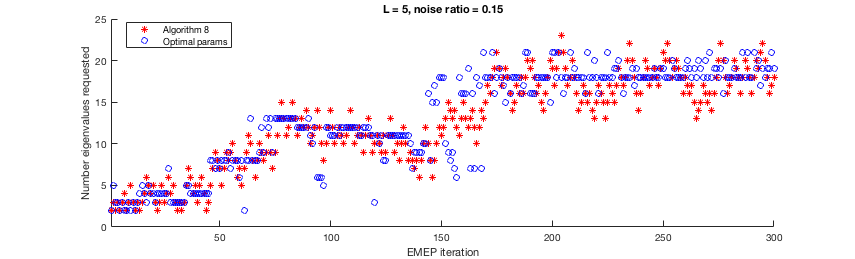
\includegraphics[scale=0.6]{Numerics-num_eigs_ada_vs_opt_1} }\vspace{0.6cm}
\vspace{0.2cm}
	\caption{
	Plot comparing Algorithm \ref{Alg:adaptive_IRAM} with the optimal choice of parameter $r$ (number of requested eigenvalues in the IRAM).
	 The \emep \ is from Figure \ref{Fig:Numerics-num_matvecs_orig_vs_optimal_params} and Arnoldi decomposition (\ref{Eqn:Arnoldi_decomp}) size is $m=40$.
	}
\label{Fig:Numerics-num_eigs_ada_vs_opt_one_plot}
\end{figure}
% experiments.figure.noisyimage_adaptive_eig_full_exp

Figure \ref{Fig:Numerics-num_eigs_ada_vs_opt_one_plot} shows that the parameter values $r_k$ chosen by Algorithm \ref{Alg:adaptive_IRAM} effectively track the optimal parameters for the IRAM.  
For the majority of iterates, the value $r_k$ is within two units from the optimal parameter value.
As we will see in Section \ref{Subsec:Numerics-correl_btwn_EMEP_and_IRAM}, these changes in $r_k$ are related to the evolving spectrum of the \emep.




 


\section{Correlation between EMEP spectrum distribution and behavior of the IRAM}
\label{Subsec:Numerics-correl_btwn_EMEP_and_IRAM}



In this section we examine an observed correlation between the clustering of the algebraically largest eigenvalues in the \emep \ and the convergence behavior of the IRAM (Algorithm \ref{Alg:IRAM}) for various parameters.
As we saw in Section \ref{Subsec:PLGD_term_crit-stagnation}, PLGD models with Gaussian noise (\ref{Eqn:PhaseLift-GD_Gaussian_noise}) typically have optimal EMEP matrices $\caA^*y_\star$ for which the algebraically largest eigenvalue has multiplicity greater than one.
Thus we may expect the algebraically largest eigenvalues in the EMEP to cluster for later iterates.

In Section \ref{Subsubsec:Numerics-correl_clustering_IRAM_param} we examine two PLGD models and show that as the eigenvalues in the EMEP begin to cluster, the \textit{optimal} IRAM parameter $\bar{r}$ (i.e., the number of requested eigenvalues $r$ with the minimum number of matrix-vector products) increases such that $\lambda_{\bar{r}+1}$ is not clustered with $\lambda_1, \lambda_2, \ldots, \lambda_{\bar{r}}$.
We also see that the value $r_k$ chosen by Algorithm \ref{Alg:adaptive_IRAM} properly tracks the optimal parameter $\bar{r}_k$ for these two PLGD models.
Next, Section \ref{Subsubsec:Numerics-default_Arnoldi_decomp_size} uses these two PLGD models to demonstrate that the Arnoldi decomposition (\ref{Eqn:Arnoldi_decomp}) size $m=40$ is sufficiently large for the IRAM to perform efficiently, and thus $m=40$ is an appropriate default parameter for Algorithm \ref{Alg:adaptive_IRAM}.





To illustrate these observations, we focus on the EMEP of two particular PLGD models with Gaussian noise (\ref{Eqn:PhaseLift-GD_Gaussian_noise}) for which the sequence of parameters $r_1, r_2, \ldots r_{maxit}$ chosen by Algorithm \ref{Alg:adaptive_IRAM} varies greatly.

\begin{figure}[H]
\centering
\hbox{\hspace{-1.8cm} 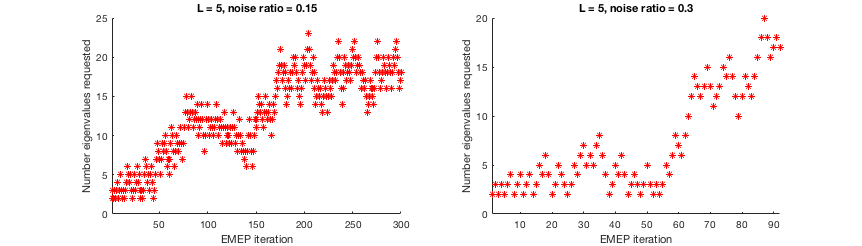
\includegraphics[scale=0.6]{Numerics-num_eigs_req_ada_2_exps} }\vspace{0.0cm}
	\caption{
Number of requested eigenvalues $r$ chosen by Algorithm \ref{Alg:adaptive_IRAM} for the \emep \ from two PLGD models with Gaussian noise (\ref{Eqn:PhaseLift-GD_Gaussian_noise}), with noise ratio $\epsilon_\text{rel}=0.15, 0.30$, oversampling rate $L=5$, and original signal from Figure \ref{Fig:parrot_signal_iterates} resized to $64 \times 64$ pixels.
}
\label{Fig:Numerics-num_req_eigs_2_exps}
\end{figure}
% experiments.figure.noisyimage_adaptive_eig_full_exp



For both PLGD models in Figure \ref{Fig:Numerics-num_req_eigs_2_exps}, changes in the EMEP caused Algorithm \ref{Alg:adaptive_IRAM} to increase the number of requested eigenvalues $r_k$ significantly from early to later iterates $k$.
Yet the value of $r_k$ increased at a quicker rate for the experiment in Figure \ref{Fig:Numerics-num_req_eigs_2_exps} with $L=5$ and $\epsilon_\text{rel} = 0.30$.
As we will see in Section \ref{Subsubsec:Numerics-correl_clustering_IRAM_param}, this quick increase from $r_{55}=3$ to $r_{70}=13$ coincides with a sudden clustering of the algebraically largest eigenvalues in the EMEP.





\subsection{Observed correlation between eigenvalue clustering and IRAM parameter choice}		\label{Subsubsec:Numerics-correl_clustering_IRAM_param}




We now show that the PLGD models in Figure \ref{Fig:Numerics-num_req_eigs_2_exps} exhibit a correlation between the spectrum distribution of the \emep \ and the convergence behavior of the IRAM (Algorithm \ref{Alg:IRAM}).
For these two models, as the algebraically largest eigenvalues $\lambda_1, \lambda_2, \ldots, \lambda_{m-1}, \lambda_{m}$ of the EMEP begin to cluster, 
the IRAM converges much faster if the number of requested eigenvalues $r<m$ is large enough such that $\lambda_{r+1}$ is not clustered with $\lambda_1, \lambda_2, \ldots, \lambda_r$.
Thus, as Algorithm \ref{Alg:adaptive_IRAM} explicitly tracks the optimal sequence of parameters $\bar{r}_k$, this algorithm implicitly tracks the clustering of the algebraically largest eigenvalues in the EMEP.
To demonstrate these observations, we consider various EMEP iterates $k$ and number of requested eigenvalues $r$, and plot the numbers of matrix-vector products for the IRAM as well as the eigenvalue difference $\lambda_{r+1} - \lambda_r$.
Figures \ref{Fig:Numerics-surf_mvs_eig_diffs_1} and \ref{Fig:Numerics-surf_mvs_eig_diffs_2} depict about half of the EMEP iterates from the two PLGD models in Figure \ref{Fig:Numerics-num_req_eigs_2_exps}, so we may focus on the regions where $r_k$ in Algorithm \ref{Alg:adaptive_IRAM} varies greatest.





\begin{figure}[H]
\centering
\hbox{\hspace{-0.5cm} 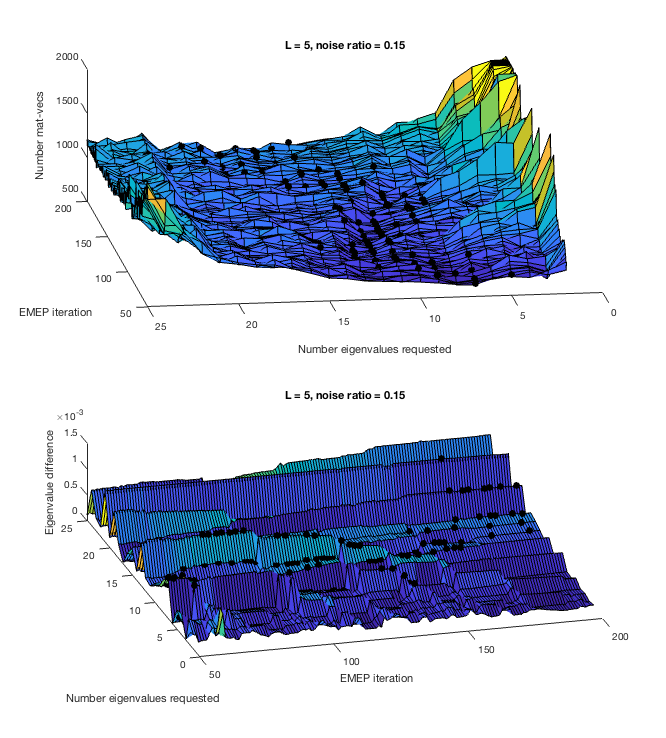
\includegraphics[scale=0.65]{Numerics-surf_num_mvs_and_eig_diffs_1} }\vspace{0.0cm}
	\caption{Behavior of Algorithm \ref{Alg:adaptive_IRAM} for the experiment from Figure \ref{Fig:Numerics-num_req_eigs_2_exps} with $L=5$, $\epsilon_\text{rel}=0.15$.  Top: Number of matrix-vector products (capped at 2,000 for better viewing) for each \emep \ iterate $k$ and number of requested eigenvalues $r$. Bottom: eigenvalue differences $\lambda_r - \lambda_{r+1}$ for each \emep \ iterate $k$ and number of requested eigenvalues $r$.  Black dots in both plots indicate the value $r_k$ chosen by Algorithm \ref{Alg:adaptive_IRAM}.}
\label{Fig:Numerics-surf_mvs_eig_diffs_1}
\end{figure}
% experiments.figure.noisyimage_adaptive_eig_full_exp



\begin{figure}[H]
\centering
\hbox{\hspace{-0.5cm} 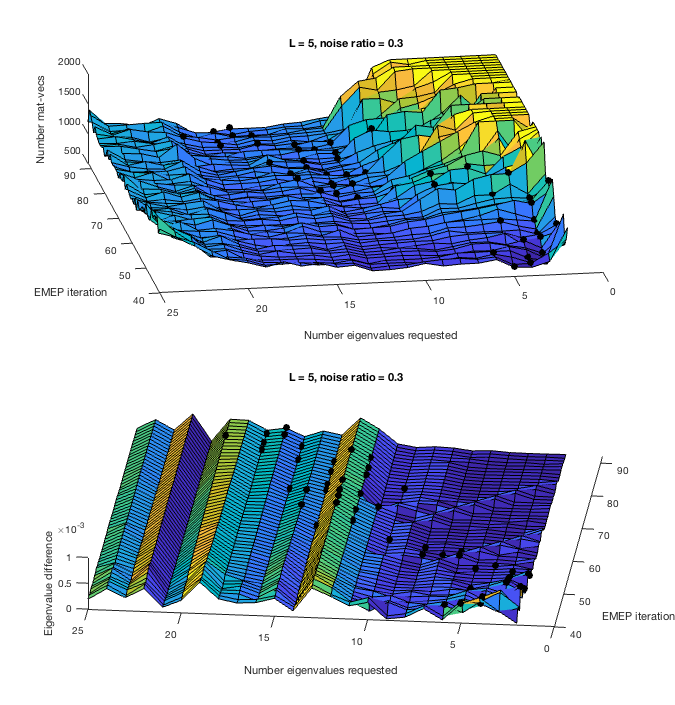
\includegraphics[scale=0.65]{Numerics-surf_num_mvs_and_eig_diffs_2} }\vspace{0.0cm}
	\caption{Behavior of Algorithm \ref{Alg:adaptive_IRAM} for the experiment from Figure \ref{Fig:Numerics-num_req_eigs_2_exps} with $L=5$, $\epsilon_\text{rel}=0.30$.  Top: Number of matrix-vector products (capped at 2,000 for better viewing) for each \emep \ iterate $k$ and number of requested eigenvalues $r$. Bottom: eigenvalue differences $\lambda_r - \lambda_{r+1}$ for each \emep \ iterate $k$ and number of requested eigenvalues $r$.  Black dots in both plots indicate the value $r_k$ chosen by Algorithm \ref{Alg:adaptive_IRAM}.}
\label{Fig:Numerics-surf_mvs_eig_diffs_2}
\end{figure}
% experiments.figure.noisyimage_adaptive_eig_full_exp





In Figures \ref{Fig:Numerics-surf_mvs_eig_diffs_1} and \ref{Fig:Numerics-surf_mvs_eig_diffs_2} we see that the clustering of the algebraically largest eigenvalues corresponds to an increase in the optimal number of requested eigenvalues $\bar{r}_k$ for later \emep \ iterates $k$.
In Figure \ref{Fig:Numerics-surf_mvs_eig_diffs_1}, the eigenvalues $\lambda_1, \lambda_2, \ldots, \lambda_{10}$ cluster around iterates $125 \leq k \leq 175$; and likewise the optimal parameter $\bar{r}_{125} \approx 10$ increases to $\bar{r}_{175} \approx 18$.
Figure \ref{Fig:Numerics-surf_mvs_eig_diffs_2} depicts a similar shift, where the eigenvalues $\lambda_1, \lambda_2, \ldots, \lambda_{10}$ cluster around iterates $50 \leq k \leq 70$, and the optimal parameter increases to $\bar{r}_{70} \approx 15$.
In the case of Figure \ref{Fig:Numerics-surf_mvs_eig_diffs_2}, the most tightly clustered eigenvalues $\lambda_1, \lambda_2, \ldots, \lambda_{8}$ also correspond to parameter values $r = 2, 3, \ldots, 7$ for which the IRAM required the greatest number of matrix-vector products to converge.



This observed correlation between eigenvalue clustering and a change in the convergence rate of the IRAM may be related to the subroutines used in the IRAM.
As discussed in Section \ref{Subsec:evol_mats-IRAM}, the IRAM is based on the following two algorithms.
Given a Hermitian matrix $A \in \bbC^{n \times n}$, the $m$-step Arnoldi iteration (Algorithm \ref{Alg:Arnoldi_iteration}) generates a set of Ritz pairs $(\theta_1, u_1), (\theta_2, u_2), \ldots, (\theta_m, u_m)$ for $A$ with respect to $\caK_m(A, q_1)$.
Next, the $p$-step shifted QR iteration (Algorithm \ref{Alg:shifted_QR_iteration}) restarts the Arnoldi decomposition (\ref{Eqn:Arnoldi_decomp}) by attempting to damp the unwanted part of the spectrum using the Ritz values $\{ \theta_{r+1}, \theta_{r+2}, \ldots, \theta_m \}$ (where $m = r + p$).
Assume we have an EMEP matrix iterate $A_k$ with some number $s$ of clustered algebraically largest eigenvalues, $\lambda_1 \approx \lambda_2 \approx \cdots \approx \lambda_s$; 
and assume we select the number of requested eigenvalues $r < s$.
When the IRAM builds an Arnoldi decomposition (\ref{Eqn:Arnoldi_decomp}), the $s$ largest Ritz values of $A_k$ with respect to $\caK_m(A_k, q_1)$ may include values $\theta_{r+1}, \theta_{r+2}, \ldots, \theta_s$ which are close approximations to the desired eigenvalues.
Thus when the shift values $\mu_1 = \theta_{r+1}, \mu_2 = \theta_{r+2}, \ldots, \mu_{s-r} = \theta_{s}, \ldots, \mu_p = \theta_m$ are passed to the $p$-step shifted QR iteration, the implicit polynomial filter (\ref{Eqn:filter_poly}) will include values $\mu_1, \mu_2, \ldots, \mu_{s-r}$ which damp the desired part of the spectrum.
Thus, if $r < s$ we may expect the IRAM to converge more slowly.
However, if we select the number of requested eigenvalues $r > s$, then the shift values used in the $p$-step shifted QR iteration will always include parts of the spectrum which we want to damp and we may expect the IRAM to converge more quickly. 


Figures \ref{Fig:Numerics-surf_mvs_eig_diffs_1} and \ref{Fig:Numerics-surf_mvs_eig_diffs_2} also demonstrate that Algorithm \ref{Alg:adaptive_IRAM} properly tracks the optimal number of requested eigenvalues $\bar{r}_k$ as this value changes.
In particular, Figure \ref{Fig:Numerics-surf_mvs_eig_diffs_2} indicates that $\bar{r}_k$ increased quickly from iterates $k = 50$ to $k = 70$.
Likewise, Algorithm \ref{Alg:adaptive_IRAM} increased $r_k$ by two units for several iterates $55 \leq k \leq 70$ (see Figure \ref{Fig:Numerics-num_req_eigs_2_exps}).
These two-unit increases were the result of Algorithm \ref{Alg:adaptive_IRAM} properly identifying a quick increase in the number of matrix-vector products $t_k$ for smaller values $r_k$.
Recall that Algorithm \ref{Alg:adaptive_IRAM} determines the update $r_{k+1}$ using two-point and four-point linear interpolations (equations (\ref{Eqn:adaptive_delta_2}) and (\ref{Eqn:adaptive_delta_4_lin_interp_prob}), respectively) of the previous parameters $r_k$ and $t_k$.
For the PLGD model in Figure \ref{Fig:Numerics-surf_mvs_eig_diffs_2}, both of these interpolations agreed (i.e., $\delta_2=1$ in (\ref{Eqn:adaptive_delta_2}) was equal to $\delta_4=1$ in (\ref{Eqn:adaptive_delta_4})) for several iterates $55 \leq k \leq 70$.
Thus Algorithm \ref{Alg:adaptive_IRAM} quickly increased $r_k$, avoiding excessive matrix-vector multiplications.







\subsection{Selecting the default Arnoldi decomposition size for the IRAM with adaptive parameter selection}		\label{Subsubsec:Numerics-default_Arnoldi_decomp_size}



Next we show that the default parameter setting $m = 40$ in Algorithm \ref{Alg:adaptive_IRAM} is sufficiently large to minimize the number of matrix-vector products in the EMEP in the models from Figure \ref{Fig:Numerics-num_req_eigs_2_exps}.
To demonstrate that $m=40$ is appropriate, we will examine a more difficult eigenvalue problem (i.e., later iterate) from each of these models.
Figure \ref{Fig:Numerics-surf_mvs_for_m_vs_j} depicts the number of matrix-vector products for various IRAM parameters $r$ and $m$ for an iterate from each model.


\begin{figure}[H]
\centering
\hbox{\hspace{-0.1cm} 
	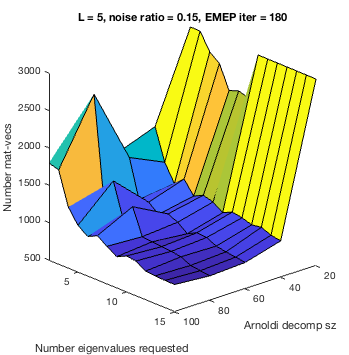
\includegraphics[scale=0.6]{Numerics-surf_mvs_for_m_vs_j_1}
	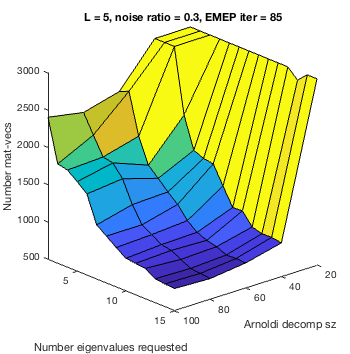
\includegraphics[scale=0.6]{Numerics-surf_mvs_for_m_vs_j_2} 
			}
	\vspace{0.0cm}
	\caption{
Number of matrix-vector products (capped at 3,000 for better viewing) for individual \emep \ iterates with varying number of requested eigenvalues $r$ and Arnoldi decomposition (\ref{Eqn:Arnoldi_decomp}) size $m$.  
Left: EMEP iterate 180 from Figure \ref{Fig:Numerics-surf_mvs_eig_diffs_1}.
Right: EMEP iterate 85 from Figure \ref{Fig:Numerics-surf_mvs_eig_diffs_2}.
	}
\label{Fig:Numerics-surf_mvs_for_m_vs_j}
\end{figure}
% experiments.figure.noisyimage_adaptive_eig_full_exp




Figure \ref{Fig:Numerics-surf_mvs_for_m_vs_j} suggests that we should not select IRAM parameters below $r = 9$ and $m = 40$ for the EMEP iterate in the left plot, nor should we select parameters below $r = 12$ and $m = 40$ for the EMEP iterate in the right plot.  
Yet there is no significant benefit to selecting larger parameter values.
Since the EMEP iterates in Figure \ref{Fig:Numerics-surf_mvs_for_m_vs_j} represent later, more difficult eigenvalue problems, this figure suggests that $m = 40$ is sufficiently large for all iterates.
Thus we select a fixed Arnoldi decomposition (\ref{Eqn:Arnoldi_decomp}) size $m = 40$ for Algorithm \ref{Alg:adaptive_IRAM}.











